\chapter{Il sistema chimico}
\vspace{0.5cm}
\label{cha:789}

Una delle proprietà fondamentali degli organismi viventi è l'abilità di sentire e rispondere ai cambiamenti dell'ambiente tramite il movimento. 
Se consideriamo la cellula, in termini generali, come un sistema chimico aperto in una situazione di non-equilibrio, è essenziale avere a disposizione un rifornimento di materiale fresco e di energia per sostenere questo sistema. Per fare in modo che questo avvenga, la cellula modifica il suo ambiente esterno metabolizzando risorse di sostentamento e producendo dei prodotti e degli scarti. Per evitare una situazione statica, di equilibrio, il sistema deve trovare in qualche modo nuove risorse da sfruttare e allo stesso tempo deve evitare gli eventuali effetti inibitori dei prodotti di scarto. In questo senso puramente chimico-biologico si crede che l'abilità di movimento giochi un ruolo importante per evitare lo stato di equilibrio nella creazione di sistemi cellulari artificiali. \cite{doi:10.1021/ja0706955}

\section{Chemiotassi e Chemiochinesi}
\label{sec:456}
Una cellula che percepisce delle molecole solubili può muoversi lungo il gradiente di concentrazione creato da queste fino a raggiungere la sorgente oppure allontanarsi da questa nel caso in cui le sostanze rilasciate siano repellenti o tossine. 
In generale, la motilità di una cellula può essere di tre tipi:
\begin{enumerate}
\item motilità basale casuale: avviene in assenza di stimoli chimici,
\item Chemiochinesi: corrisponde ad un movimento casuale in aumento, in risposta a stimoli chimici
\item Chemiotassi: migrazione stimolata verso un gradiente chimico.
\end{enumerate}
La \emph{chemiotassi} può essere di tipo positivo in caso di avvicinamento alla sorgente e di tipo negativo in caso di allontanamento.
	\begin{figure}[h]
	  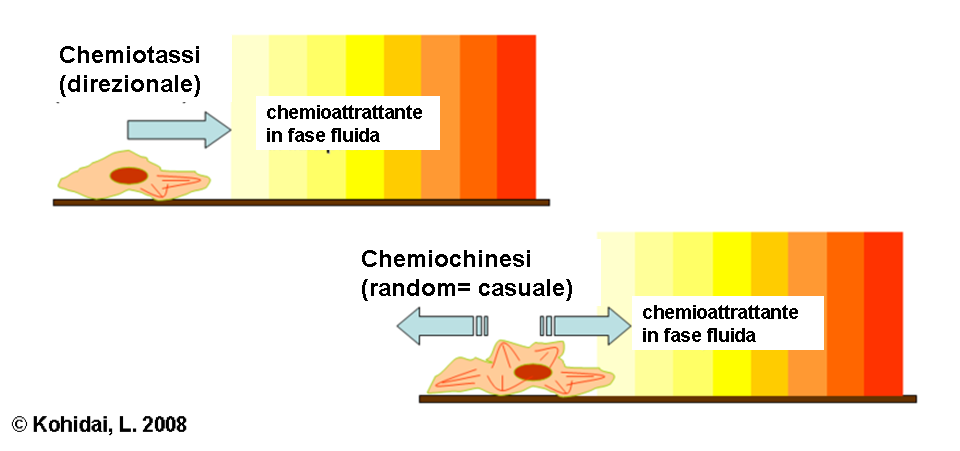
\includegraphics[scale=0.60]{immagini/chemochin.png}
		\centering	
	 \caption{chemiotassi e chemiochinesi}
	\end{figure}
\\In questo studio ci si sofferma sul movimento chemiotattico positivo promosso da una \emph{droplet} di decanolo in acido decanoico lungo il gradiente di concentrazione creato dall'aggiunta di cloruro di sodio.
\subsection{L'importanza del movimento}
\label{sec:00456}

\begin {itemize}
	\item nutrimento di cellule singole e sopravvivenza + 
	\item condizioni di malattia e di salute
	\item trasporto di cargo
\end{itemize}

\section{Componenti inorganiche}
\label{sec:123}
Durante il progetto è stato implementato un programma per la gestione di un sistema chimico composto da una \emph{droplet} di decanolo che si muove in una soluzione acquosa di acido decanoico $(C_{10}H_{20}O_{2})$ lungo i gradienti di concentrazione formati con l'aggiunta di cloruro di sodio $(NaCl)$. 



